%!Mode:: "TeX:UTF-8"
\section{死锁}


死锁产生的现场:当A进程P S2信号量而B进程P S1信号量时就会产生死锁,因为S2信号量需要B进程释放,而S1信号量需要A进程释放,因此两个进程都在等相互的资源,造成死锁。

\begin{figure}[ht]
	\begin{center}
		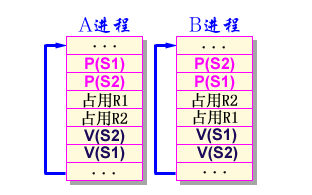
\includegraphics[keepaspectratio,width=0.5\paperwidth]{Pictures/deadlock.png}
	\caption{死锁示例}
	\label{fig:deadlock}
	\end{center}
\end{figure}

死锁产生的条件:
\begin{itemize}
\item  
互斥条件:进程要求对所分配的资源进行排它性控制,即在一段时间内某资源仅为一进程所占用。(信号量s1 s2为互斥的信号量,只能被一个进程占用)
\item  
请求和保持(部分分配,占有申请):已持有资源的进程可以请求新资源(A进程在获取s2阻塞时,一直占用s1)
\item  
不可剥夺条件:进程已获得的资源在未使用完之前,不能剥夺,只能在使用完时由自己释放。(s1只能由A进程释放,s2只能由B进程释放)
\item  
环路等待条件:在发生死锁时,必然存在一个进程--资源的环形链。(A B 进程都是环形链路)
\end{itemize}

为避免死锁,可以从上述后三个条件入手,而第一个互斥条件是无法被破坏的\cite{pibible}。

银行家算法(Banker's Algorithm)是一个避免死锁(Deadlock)的著名算法,是由Edsger Dijkstra 在1965年为T.H.E系统设计的一种避免死锁产生的算法。它以银行借贷系统的分配策略为基础,判断并保证系统的安全运行。

如果所有过程有可能完成执行(终止),则一个状态(如上述范例)被认为是安全的。由于系统无法知道什么时候一个过程将终止,或者之后它需要多少资源,系统假定所有进程将最终试图获取其声明的最大资源并在不久之后终止。在大多数情况下,这是一个合理的假设,因为系统不是特别关注每个进程运行了多久(至少不是从避免死锁的角度)。此外,如果一个进程终止前没有获取其它能获取的最多的资源,它只是让系统更容易处理。


基于这一假设,该算法通过尝试寻找允许每个进程获得的最大资源并结束(把资源返还给系统)的进程请求的一个理想集合,来决定一个状态是否是安全的。不存在这个集合的状态都是不安全的。如果一个资源请求无法被满足,则驳回。如果该请求key被满足,但导致系统离开了安全状态,则该请求不被受理,即延缓执行或驳回。
